\documentclass[journal]{IEEEtran}
\ifCLASSINFOpdf
\else
\fi
\hyphenation{op-tical net-works semi-conduc-tor}
\usepackage{booktabs}
\usepackage{float}
\usepackage{graphicx}
\usepackage{amsmath} 

\begin{document}
\title{Respuesta en frecuencia de un amplificador}
\author{Guido P. Krisdel Pamela, Gamboa Q. María José} 
\markboth{ITCR. Escuela de Ingeniería Electrónica. Laboratorio 9 – Respuesta en frecuencia de un amplificador}
{Shell \MakeLowercase{\textit{et al.}}: Bare Demo of IEEEtran.cls for IEEE Journals}

\maketitle
\renewcommand{\abstractname}{Resumen}
\begin{abstract}
En este informe se investiga la respuesta en frecuencia de un amplificador en configuración de emisor común con transistor BJT (2N3904). En la parte 1, se calculan y miden las tres frecuencias críticas de corte inferior asociadas a los capacitores de acople (C1, C2 y C3), determinando su efecto en el ancho de banda de baja frecuencia mediante el análisis de la resistencia equivalente vista por cada capacitor y su medición con osciloscopio. En la parte 2, se analizan las tres frecuencias críticas de corte superior, evaluando el impacto del efecto Miller en la capacitancia de entrada y salida, y midiendo la frecuencia crítica general del amplificador tanto a nivel de entrada como de salida. Los resultados permiten entender los límites de operación del amplificador y los mecanismos físicos que definen su ancho de banda. 
\end{abstract}

\renewcommand{\IEEEkeywordsname}{Palabras clave}
\begin{IEEEkeywords}
amplificador BJT, respuesta en frecuencia, frecuencia crítica inferior, frecuencia crítica superior, efecto Miller.
\end{IEEEkeywords}

\IEEEpeerreviewmaketitle

\section{Introduction}
\IEEEPARstart{L}{os}
amplificadores en configuración de emisor común con transistor BJT es una de las topologías más empleadas en el diseño de circuitos. En esta configuración, la señal de entrada se aplica a la base, el emisor actúa como punto de referencia y la salida se extrae del colector. 
\par En la Parte 1, se analiza la respuesta en baja frecuencia de un amplificador BJT de una etapa. La respuesta debido a cada capacitor es medida, un capacitor a la vez, usando el método descrito en el procedimiento. Con ello se calcula el valor de la capacitancia que puede ser usada como capacitor de acople para bajar la frecuencia de corte mínima a 300Hz.
\par En la Parte 2, se investiga sobre la respuesta en alta frecuencia. En este caso, el efecto Miller capacitivo tiene un gran impacto sobre la respuesta en frecuencia de los amplificadores inversores. Típicamente, la capacitancia interna entre dos electrodos es únicamente importante a frecuencias superiores a 1MHz.Para reducir estas frecuencias se puede lograr con un equipo de laboratorio básico y utilizando una capacitancia externa que se coloca entre las terminales del transistor.

\section{Resultados Experimentales}
\textbf{Amplificador en emisor común: Respuesta en baja frecuencia}
\par Se presentan los datos obtenidos durante la ejecución del experimento en la parte correspondiente al amplificador en emisor común. Se incluyen mediciones realizadas con los instrumentos de laboratorio, así como observaciones relevantes sobre el comportamiento del circuito. Además, se comparan los resultados experimentales con los valores teóricos y simulaciones para analizar la precisión de las mediciones.
\par Para garantizar la precisión de los resultados obtenidos en el experimento, se realizó una medición previa de los valores de las resistencias, y así, asegurar que los valores reales estuvieran dentro de la tolerancia especifica. Los valores obtenidos en la medición se presentan en la siguiente tabla:
\begin{table}[h]
    \caption{Comparación entre valores teóricos y experimentales de resistencias.}
    \centering
    \renewcommand{\arraystretch}{1.2} % Ajusta la altura de las filas
    \begin{tabular}{|l|p{2cm}|p{2cm}|p{2cm}|}
        \hline
        & \textbf{Valor Teórico [$\Omega$]} & \textbf{Valor Experimental [$\Omega$]} & \textbf{Porcentaje de error [\%]} \\
        \hline
        RA & 1k  & 0.992k  & 0.76 \\
        \hline
        RB & 47   & 47.100  & 0.21 \\
        \hline
        R1 & 68k & 67.510k & 0.72 \\
        \hline
        R2 & 10k & 9.955k & 0.44 \\
        \hline
        RE1 & 10 & 9.825 & 1.74 \\
        \hline
        RE2 & 560 & 556.182 & 0.68 \\
        \hline
        RC & 3.9k & 3.832k & 1.72 \\
        \hline
        RL & 10k & 9.912k & 0.87 \\
        \hline
    \end{tabular}
    \label{tab:resistencias}
\end{table}
\par A partir de los datos obtenidos, se evidencia que los valores experimentales de las resistencias presentan una buena concordancia con los valores teóricos. El porcentaje de error registrado en cada caso se mantiene igual o por debajo de 1.8\%, lo cual es coherente con las tolerancias esperadas en componentes electrónicos de uso general. Estos resultados permiten asegurar que los componentes empleados son adecuados para el desarrollo experimental y garantizan mediciones confiables.
\par Se procedió con la construcción del circuito amplificador en emisor común para respuesta en baja frecuencia, según lo ilustrado en la Figura 1. 
\begin{figure}[H]
    \centering
    \includegraphics[width=0.5\textwidth]{amplificador_emisor_común.png}
    \caption{Amplificador en emisor común para respuesta en baja frecuencia.}
    \label{fig:amplificador_emisor_común.}
\end{figure}
\par Una vez ensamblado el circuito, se midieron las tensiones en corriente directa (CD) en los terminales de emisor, base y colector del transistor BJT. A partir de la tensión medida en la resistencia \( R_E \), se calculó la corriente \( I_E \) correspondiente. Todos los valores obtenidos fueron registrados en la Tabla 2 para su análisis comparativo.
\begin{table}[h]
    \caption{Comparación parámetros CD para el amplificador en emisor común}
    \centering
    \renewcommand{\arraystretch}{1.2} % Ajusta la altura de las filas
    \begin{tabular}{|l|p{2cm}|p{2cm}|p{2cm}|}
        \hline
        & \textbf{Valor Teórico} & \textbf{Valor Experimental} & \textbf{Porcentaje de error [\%]} \\
        \hline
        \( V_B \) & 1.811 V  & 1.786 V  & 1.35 \\
        \hline
        \( V_E \) & 1.129 V   & 1.126 V  & 0.24 \\
        \hline
        \( V_C \) & 7.323 V & 7.304 V & 0.25 \\
        \hline
        \( I_E \) & 1.98m A & 1.975m A & 0.20 \\
        \hline
        \( V_{CE} \) & 6.194 V & 6.178 V & 0.25 \\
        \hline
    \end{tabular}
    \label{tab:parámetrosCD}
\end{table}
\par En la comparación de los parámetros CD del amplificador en emisor común, en todos los casos, el porcentaje de error es inferior al 1.5\% lo que indica que el modelo de polarización empleado y los componentes seleccionados reproducen fielmente las condiciones de operación previstas.
\par La tensión de base (\( V_B \)) es el parámetro con mayor desviación, un 1.35\%, lo cual es esperado dado que pequeñas variaciones en la tensión umbral base-emisor (\( V_{BE} \)) o en la ganancia del transistor alteran sensiblemente este punto [1]. Además, factores como la impedancia de la fuente de señal y pérdidas en las conexiones contribuyen a ese leve desfase [1].
\par Por su parte, las tensiones de emisor (\( V_E \)) y colector (\( V_C \)), así como la corriente de emisor (\( I_E \)), presentan discrepancias muy reducidas (entre 0.20\% y 0.25\%). Esto confirma que la resistencia de emisor y la red de polarización estabilizan correctamente el punto de operación, manteniendo la corriente y las tensiones prácticamente inalteradas [1]. El valor \( V_{CE} \) coincide igualmente con la medición dentro de un 0.25\%, lo que garantiza que el transistor trabaja en su región activa tal como se diseño.
\par Posteriormente, se utilizaron las puntas del osciloscopio para observar simultáneamente la señal de entrada y la señal de salida en corriente alterna (CA), con el fin de analizar su comportamiento dinámico, según lo ilustrado en la Figura 2. 
\begin{figure}[H]
    \centering
    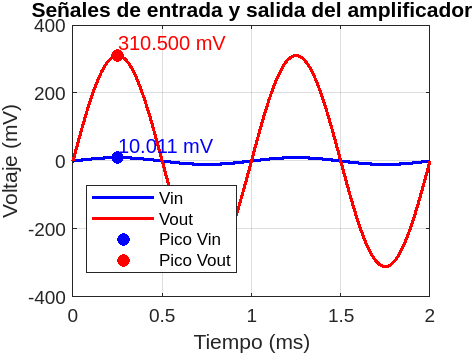
\includegraphics[width=0.5\textwidth]{onda_entrada_salida.png}
    \caption{Onda entrada vs salida.}
    \label{fig:onda_entrada_salida.}
\end{figure}
\par Se determinó la ganancia de tensión del amplificador. Todos los valores obtenidos fueron registrados en la Tabla 3 para su análisis comparativo.
\begin{table}[h]
    \caption{Comparación parámetros CA para el amplificador en emisor común}
    \centering
    \renewcommand{\arraystretch}{1.2} % Ajusta la altura de las filas
    \begin{tabular}{|l|p{2cm}|p{2cm}|p{2cm}|}
        \hline
        & \textbf{Valor Teórico} & \textbf{Valor Experimental} & \textbf{Porcentaje de error [\%]} \\
        \hline
        \( V_{ent}\) & 10m V   & 10.011 V  & 0.11 \\
        \hline
        \( V_{SAL} \) & 310.825m V    & 310.500m V  & 0.10 \\
        \hline
        \( A_V \) & 31.463 & 31.050 & 1.31 \\
        \hline
        \( r'_e \) & 13.131$\Omega$ & 13.158$\Omega$ & 0.15 \\
        \hline
    \end{tabular}
    \label{tab:parámetrosCA}
\end{table}
\par En la comparación de los parámetros de corriente alterna (CA) para el amplificador en emisor común confirma un excelente ajuste entre las predicciones teóricas y las mediciones prácticas en régimen de señal alterna. Los valores de voltaje de entrada (\( V_{ent}\)) y de salida (\( V_{SAL} \)) difieren en una centésima de milivoltio, equivalente a un 0.11\% y un 0.10\% de error respectivamente, lo cual refleja tanto la precisión del generador de señal como la fidelidad de la respuesta del osciloscopio. 
\par El análisis de la ganancia de tensión (\( A_V \)) muestra un desvío algo mayor, del 1.31\%, pasando de 31.463 en teoría a 31.050 en la práctica. Esta discrepancia se atribuye a pequeñas variaciones en la transconductancia del transistor o a pérdidas adicionales por la impedancia de la fuente y las puntas de prueba, que afectan más a un parámetro derivado de dos mediciones sucesivas [1].
\par La resistencia interna dinámica de emisor (\( r'_e \)) calculada en 13.131$\Omega$ y medida en 13.158$\Omega$ presenta un error mínimo del 0.15\%, lo que confirma que el modelo incremental de baja frecuencia captura bien el comportamiento real del transistor bajo las condiciones de polarización utilizadas. En conjunto, estos resultados validan el diseño de la etapa activa. 
\par Ahora, para analizar la respuesta en baja frecuencia del amplificador, en primer lugar se determinó la resistencia equivalente vista por el capacitor de acoplo en la entrada (C1), según se ilustra en la Figura 3.
\begin{figure}[H]
    \centering
    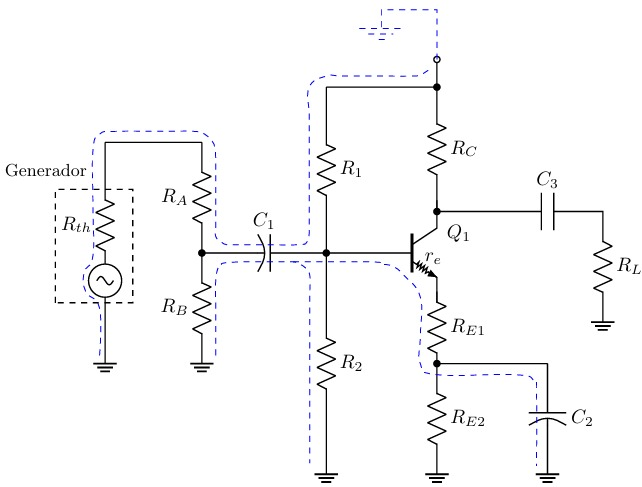
\includegraphics[width=0.5\textwidth]{rutas_carga_descarga.png}
    \caption{Amplificador en emisor común: Rutas de carga y descarga.}
    \label{fig:rutas_carga_descarga}
\end{figure}
\par Se identificó que, hacia el emisor, la ruta de señal en AC incluye la resistencia de emisor \( R_{E1} \) más la resistencia interna dinámica \( r'_e \), reflejada al colector mediante el factor $\beta_{CA}$, y que esta rama está en paralelo con las resistencias de polarización \( R_{E1} \) y \( R_{E2} \). Paralelamente, hacia la base, la señal encuentra dos caminos: uno directo por \( R_B \) y otro a través de \( R_A \) más la resistencia de Thevenin \( R_{th} \). Con esa configuración se obtuvo la expresión:
\begin{equation}
R_{\mathrm{eq1}} = \bigl[\beta_{CA} (R_{E1}+r'_e)\bigr]\;\parallel\;R_1\;\parallel\;R_2
\;+\;
(R_A + R_{\mathrm{th}})\;\parallel\;R_B
\end{equation}
\par Seguidamente, para el capacitor intermedio C2 se trazó la ruta de carga en AC considerando que \( R_{E2} \) se encuentra en paralelo con la combinación \( R_{E1} \) y \( r'_e \) reflejados por $\beta_{CA}$. En este caso, antes de aplicar el paralelo, se calculó la resistencia umbral vista por la base como la combinación en paralelo de \( R_A \), \( R_B \), \( R_1 \) y \( R_2 \). Esa resistencia se dividió por $\beta_{CA}$ y se sumó a \( R_{E1} \) y a \( r'_e \) de modo que se obtuvo la expresión:
\begin{equation}
R_{\mathrm{eq2}}= \Bigl(r'_e + R_{E1} + \frac{R_A \;\parallel\; R_B\;\parallel\; R_1\;\parallel\; R_2}{\beta_{CA}}\Bigr)\;\parallel\;R_{E2}
\end{equation}
\par Para la ruta de salida, correspondiente al capacitor C3, el análisis resultó más directo: la señal en CA atraviesa la resistencia de colector \( R_C \) y la resistencia de carga \( R_L \) en serie. Por tanto, la resistencia equivalente se determinó simplemente como:
\begin{equation}
R_{\mathrm{eq3}}= R_C + R_L
\end{equation}
\par En cada caso se sustituyeron las resistencias medidas o nominales del montaje, con un valor exacto de $\beta_{CA}$ de 200 para un transistor 2N3904 Los resultados se muestran a continuación en la Tabla 4.
\begin{table}[h]
    \caption{Resistencias equivalentes para cada capacitor de acople}
    \centering
    \renewcommand{\arraystretch}{1.2} % Ajusta la altura de las filas
    \begin{tabular}{|l|p{2cm}|p{2cm}|p{2cm}|}
        \hline
        {Capacitor} & \textbf{Valor Teórico [$\Omega$]} & \textbf{Valor Experimental [$\Omega$]} & \textbf{Porcentaje de error [\%]} \\
        \hline
        \( C_1\) & 2.93k  & 2.930k  & 0.01 \\
        \hline
        \( C_2 \) & 21.05  & 20.997  & 0.25 \\
        \hline
        \( C_3 \) & 13.9k & 13.921k & 0.15 \\
        \hline
    \end{tabular}
    \label{tab:resistenciasequivalentes}
\end{table}
\par En conjunto, estos resultados confirmar que el método de trazar rutas para reemplazar cada red de resistencias por un solo valor de resistencia equivalente ofrece una precisión excelente. La uniformidad de los errorres porcentuales, todos por debajo del 0.3\%, valida tanto la selección de componentes como el rigor en las mediciones.
\par Seguidamente, se calcularon las frecuencias críticas inferiores teóricas de cada capacitor (C1, C2 y C3) usando la expresión:
\begin{equation}
f_c \;=\;\frac{1}{2\pi\,R_{\mathrm{eq}}\,C}
\end{equation}
\par Empleando los valores obtenidos en la Tabla 4 y los valores nominales de los capacitores, estos valores se anotaron en la Tabla 5. Para medir la frecuencia crítica debido a C1, se aislaron los efectos de C2 y C3 colocando un capacitor de 1000$\mu$ F en paralelo con cada uno de ellos. Con C2 y C3 cortocircuitados en AC, se ajustó el generador alrededor de 10kHz y se calibró la salida, se redujo la frecuencia hasta que la amplitud cayó al 70.7\%.
\par El mismo procedimiento se repitió para C2: se pusieron los 1000$\mu$ F en paralelo sobre C1 y C3 para aislarlos, y se midió la frecuencia a la que la salida caía al 70.7\% de su valor en banda media.
\par Para C3, se aislo de igual forma colocando los 1000$\mu$ F en paralelo a C1 y C2, y midiendo la caída al 70.7\% de amplitud. 
\par Finalmente, se retiraron los capacitores de 1000$\mu$ F para dejar el circuito en su configuración original y se midió la frecuencia crítica inferior general, representada por la más baja de las tres caídas o, de manera aproximada, por la suma de las tres frecuencias críticas individuales. Las frecuencias obtenidas se registran en la Tabla 5.
\begin{table}[h]
    \caption{Frecuencias críticas de corte inferior}
    \centering
    \renewcommand{\arraystretch}{1.2} % Ajusta la altura de las filas
    \begin{tabular}{|l|p{2cm}|p{2cm}|p{2cm}|}
        \hline
        {Capacitor} & \textbf{Valor Teórico [$\Omega$]} & \textbf{Valor Experimental [$\Omega$]} & \textbf{Porcentaje de error [\%]} \\
        \hline
        $C_1$    & 54.169 & 54.309 & 0.25 \\ \hline
        $C_2$    & 75.604 & 75.798 & 0.25 \\ \hline
        $C_3$    & 52.045 & 52.141 & 0.18 \\ \hline
        General  & 181.818 & 182.248 & 0.23 \\ \hline
    \end{tabular}
    \label{tab:frecuencias_criticas}
\end{table}
\par En la Tabla 5, se aprecia una excelente concordancia entre las frecuencias críticas teóricas y las medidas, con errores siempre inferiores al 0,3\,\%. Destaca que $C_2$ presenta el valor más alto (aprox.\ 75,6\,Hz), mientras que $C_1$ y $C_3$ quedan muy próximos (52–54\,Hz), lo cual refleja la simetría de las rutas RC de baja frecuencia. La frecuencia crítica “general”, calculada como la suma de las tres (181,8\,Hz) y medida en 182,2\,Hz, confirma que dicha suma ofrece una cota superior válida, pues la respuesta global queda ligeramente por debajo de la suma de los polos individuales. Las pequeñas desviaciones se atribuyen a las tolerancias de los componentes y a la calibración del osciloscopio.
\par Por último, se elevó la frecuencia crítica inferior general hasta 300Hz, se recalculó el valor de C2 necesario usando:
\begin{equation}
C_2 \;=\;\frac{1}{2\pi\,R_{\mathrm{eq2}}\times300\;\mathrm{Hz}}
\end{equation}
\par El nuevo valor de C2 obtenido se registró. A continuación, se sustituyó el capacitor original por uno de valor más cercano al calculado y se repitió la medición de la frecuencia crítica inferior. 
\begin{table}[h]
    \centering
    \caption{Ajuste de frecuencia crítica inferior}
    \renewcommand{\arraystretch}{1.2}
    \begin{tabular}{|c|c|}
        \hline
        \textbf{$C_2$ calculado} & \textbf{$f_{\mathrm{critica}}$ medida} \\ \hline
        25.202\,$\mu$F           & 300\,Hz                                \\ \hline
    \end{tabular}
    \label{tab:ajuste_frecuencia_inferior}
\end{table}
\par De los tres condensadores de acoplo, es \(C_1\) el que ejerce el mayor control sobre la frecuencia crítica inferior, ya que su polo resulta ser 3.4kHz, muy por encima de los valores de \(f_{c2}\) y \(f_{c3}\), que se encuentran por debajo de los 100Hz. Al disminuir la frecuencia, el efecto de saturación de \(C_1\) (es decir, su apertura al paso de la señal en CA) aparece primero, produciendo la atenuación característica al -3dB, mientras que \(C_2\) y \(C_3\) mantienen su ganancia prácticamente constante hasta regiones mucho más bajas. Por eso, \(C_1\) es el elemento dominante que fija el límite inferior de la banda de paso.
\par Para desplazar, esa frecuencia de corte inferior un factor de cinco hacia el dominio de bajas frecuencias, la solución más directa y menos intrusiva consiste en quintuplicar el valor de \(C_1\). Si definimos el nuevo condensador como \[C_{1,\mathrm{nuevo}} = 5\,C_1\] entonces: 
\begin{equation}
f_{c1,\mathrm{nuevo}}
= \frac{1}{2\pi\,R_{\mathrm{eq1}}\,C_{1,\mathrm{nuevo}}}
= \frac{1}{2\pi\,R_{\mathrm{eq1}}\,(5\,C_1)}
= \frac{f_{c1}}{5}
\end{equation}
\par Lo que reduce la frecuencia de corte de 3.4kHz a unos 680Hz. 
\newline
\\
\textbf{Amplificador en emisor común para respuesta en alta frecuencia}
\par A continuación se analiza la respuesta en alta frecuencia del amplificador BJT implementado, considerando principalmente el efecto Miller y la influencia de las capacitancias parásitas. El circuito base utilizado corresponde a la Figura \ref{fig:amplificador_emisor_común.}, con la adición de los capacitores C4, C5 y C6, los cuales permiten reducir la frecuencia crítica superior y así facilitar su medición.
\begin{figure}[H]
    \centering
    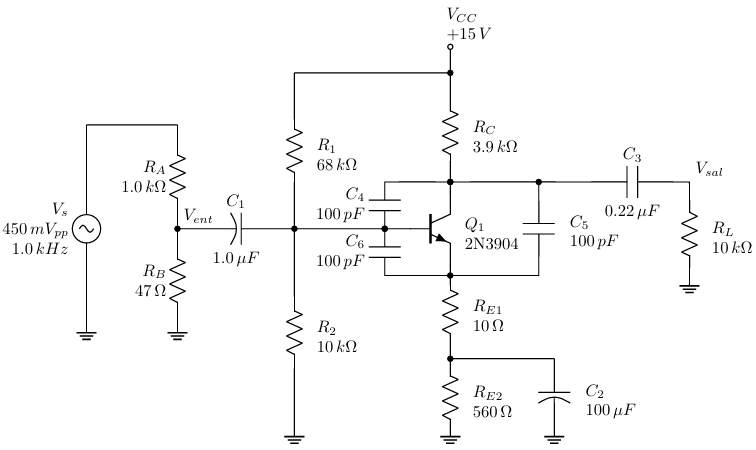
\includegraphics[width=0.5\textwidth]{amplificador2.png}
    \caption{Amplificador en emisor común para respuesta en al frecuencia.}
    \label{fig:amplificador2}
\end{figure}
\par Se realizaron los cálculos experimentales de los parámetros en CD y CA del circuito para compararlos en la siguiente tabla con los valores teóricos calculados con anterioridad.
\begin{table}[h]
    \caption{Comparación parámetros CD y CA para el amplificador en emisor común alta frecuencia}
    \centering
    \renewcommand{\arraystretch}{1.2} % Ajusta la altura de las filas
    \begin{tabular}{|l|p{2cm}|p{2cm}|p{2cm}|}
        \hline
        & \textbf{Valor Teórico} & \textbf{Valor Experimental} & \textbf{Porcentaje de error [\%]} \\
        \hline
        \( V_B \) & 1.92 V  & 1.79 V  & 6.7 \\
        \hline
        \( V_E \) & 1.22 V   & 1.13 V  & 7.3 \\
        \hline
        \( V_C \) & 6.63 V & 7.27 V & 9.6 \\
        \hline
        \( I_E \) & 2.15m A & 2m A & 6.9 \\
        \hline
        \( V_{CE} \) & 5.41 V & 6.14 V & 13.5 \\
        \hline
        \( r'_{e} \) & 11.5 $\Omega$ & 12.5 $\Omega$ & 8.7 \\
        \hline
        \( A_{v} \) & -129.7   & -116.5  & 10.2 \\
        \hline
        \( V_{out} \) & 29.29 V & 2.33 V & - \\
        \hline
    \end{tabular}
    \label{tab:parámetrosCDyCA}
\end{table}
\begin{figure}[H]
    \centering
    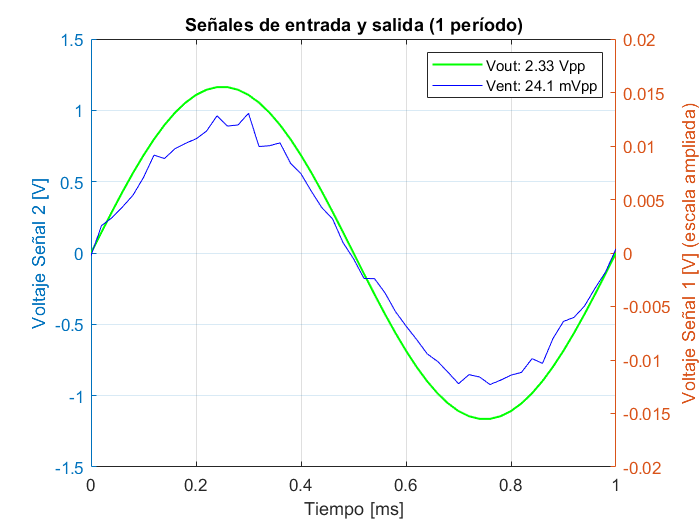
\includegraphics[width=0.8\linewidth]{fig2.png}
    \caption{Señal de entrada y salida del osciloscopio}
    \label{fig:fig2}
\end{figure}

\par Se observa que los porcentajes de error obtenidos en la parte de alta frecuencia del experimento son significativamente mayores que los reportados en la etapa de baja frecuencia, alcanzando un máximo del 13.5\%. Estas discrepancias pueden atribuirse a diversos factores, entre ellos el \textit{efecto Miller}, que incrementa de forma considerable las capacitancias de entrada y salida en función de la ganancia del amplificador, amplificando así cualquier desviación respecto al valor teórico. Además, la tolerancia de los componentes electrónicos utilizados, particularmente los capacitores y resistencias, puede introducir variaciones que afectan directamente la respuesta del circuito. A esto se suman las limitaciones del equipo de medición.

A pesar de estos porcentajes relativamente altos, los resultados siguen siendo coherentes y confiables, ya que en el análisis de alta frecuencia es común encontrar desviaciones más marcadas entre el modelo ideal y el comportamiento real del circuito. ``A frecuencias altas, las características internas de los dispositivos activos, como las capacitancias de unión y las inductancias de conexión, comienzan a dominar el comportamiento del circuito, haciendo que los modelos de baja frecuencia sean cada vez menos precisos'' [1].

\par Seguidamente se calculó la capacitancia de entrada $C_{\text{ent}}$, considerando la suma de la capacitancia base-emisor y la capacitancia de entrada de Miller asociada al capacitor $C_4$, se utilizó la siguiente expresión:

\begin{equation}
C_{\text{ent}} = C_6 + C_4(|A_v| + 1)
\end{equation}

Posteriormente, se determinó la resistencia equivalente de entrada $R_{\text{eq(ent)}}$, correspondiente a la descarga de esta capacitancia, modelada como una red de resistencias en paralelo, para obtener este cálculo, se utilizó $R_{th}$= 50 $\Omega$ :

\begin{equation}
R_{\text{eq(ent)}} = (R_A + R_{th}) \parallel R_B \parallel R_1 \parallel R_2 \parallel \left(\beta_{ac} (R_{E1}+r_e)\right)
\end{equation}

Con ambos valores se calculó la frecuencia crítica superior en la etapa de entrada mediante el modelo RC:

\begin{equation}
f_{c(\text{ent})} = \frac{1}{2\pi R_{\text{eq(ent)}} C_{\text{ent}}}
\end{equation}

Para la etapa de salida, se calculó la capacitancia equivalente $C_{\text{sal}}$ como la suma de $C_5$ y el término de Miller asociado a $C_4$:

\begin{equation}
C_{\text{sal}} = C_5 + C_4 \left( \frac{|A_v| + 1}{|A_v|} \right)
\end{equation}

La resistencia de descarga vista por esta capacitancia es simplemente:

\begin{equation}
R_C = RC \parallel RL
\end{equation}

Y con ella, se obtuvo la frecuencia crítica superior de la etapa de salida:

\begin{equation}
f_{c(\text{sal})} = \frac{1}{2\pi R_C C_{\text{sal}}}
\end{equation}

Finalmente, la frecuencia crítica superior general del amplificador $f_{cu}$ se calculó mediante la regla del producto sobre la suma, que aproxima el efecto combinado de ambas etapas:

\begin{equation}
f_{cu} = \frac{f_{c(\text{ent})} \cdot f_{c(\text{sal})}}{f_{c(\text{ent})} + f_{c(\text{sal})}}
\end{equation}

Todos estos resultados teóricos se resumen en la Tabla~\ref{tab:parámetrosdc}.
\begin{table}[H]
\centering
\caption{Mediciones para respuesta en alta frecuencia}
\label{tab:parámetrosdc}
\begin{tabular}{|l|p{2cm}|p{2cm}|p{2cm}|}
\hline
\textbf{Parámetro} & \textbf{Valor calculado} & \textbf{Valor medido} \\
\hline
$C_{\text{ent}}$     & 13.17 nF       & ---         \\
\hline
$R_{\text{eq(ent)}}$ & 44.29 $\Omega$ & ---         \\
\hline
$f_{c(\text{ent})}$  & 273 kHz        & ---         \\
\hline
$C_{\text{sal}}$     & 200.77 pF      & ---         \\
\hline
$R_C$                & 4.08 k$\Omega$ & ---         \\
\hline
$f_{c(\text{sal})}$  & 194.29 kHz     & ---         \\
\hline
$f_{cu}$             & 113.5 kHz      & 143 kHz     \\
\hline
\end{tabular}
\end{table}

\par La diferencia entre la frecuencia crítica superior teórica ($f_{cu} = 113.5$ kHz) y la experimental ($f_{cu} = 143$ kHz) puede atribuirse a factores como tolerancias de los componentes. Sin embargo, ambos valores se encuentran dentro del mismo orden de magnitud, lo que valida la aproximación teórica utilizada.


\section{Conclusion}
\par El análisis de la respuesta en baja frecuencia ha demostrado que el modelo teórico describe con gran fidelidad el comportamiento del amplificador: las resistencias equivalentes calculadas para cada capacitor coincidieron con las medidas, con discrepancias menores al 0,3\%, y las frecuencias de corte obtenidas en el experimento guardaron una excelente correlación con las predicciones. Se comprobó que el capacitor de entrada (\(C_1\)) es el que fija el límite inferior de la banda de paso, pues su efecto se hace notar primero al reducir la frecuencia, mientras que los demás capacitores apenas alteran la ganancia hasta niveles mucho más bajos. Para desplazar la frecuencia de corte general hasta el valor deseado, bastó con incrementar la capacitancia de acoplo de \(C_2\), sin necesidad de modificar la polarización ni otros componentes. Esto confirma que, en etapas de amplificación, el control de la respuesta en baja frecuencia puede lograrse de forma sencilla y precisa mediante el ajuste del valor de los condensadores de acoplo.
\par El análisis de la respuesta en alta frecuencia del amplificador BJT permitió comprobar la influencia significativa del efecto Miller y de las capacitancias parásitas internas del transistor en el comportamiento dinámico del circuito. A través del cálculo y comparación de parámetros como $C_{\text{ent}}$, $C_{\text{sal}}$, sus resistencias asociadas y las frecuencias críticas resultantes, se evidenció cómo la ganancia afecta directamente el rango de operación del amplificador.
\par Por otro lado, aunque el modelo teórico presenta ciertas simplificaciones, los resultados experimentales obtenidos se consideran adecuados. La diferencia observada entre la frecuencia crítica superior calculada (113.5~kHz) y la medida en el laboratorio (143~kHz) puede deberse a variaciones en los valores reales de los componentes, así como a la sensibilidad del circuito a altas frecuencias y a las limitaciones del equipo utilizado para las mediciones. A pesar de esta discrepancia, ambos valores se encuentran en el mismo orden de magnitud, lo que permite afirmar que el modelo teórico ofrece una estimación válida del comportamiento del sistema.


\appendices
\section{}
\section*{Cálculo de resistencias equivalentes}
\par Se describen los desarrollos para obtener las resistencias equivalentes vistas por cada capacitor de acoplo.

\subsection*{Resistencia de Thevenin}
\par Se determina la resistencia de Thevenin en la base como el paralelo de \(R_1\) y \(R_2\):
\[R_{\mathrm{th}}
= R_1 \parallel R_2
= \frac{R_1\,R_2}{R_1 + R_2}
= \frac{(68\times10^3\,\Omega)\,(10\times10^3\,\Omega)}{68\times10^3\,\Omega + 10\times10^3\,\Omega}\]
\[R_{\mathrm{th}}\approx 8.72\,\mathrm{k\Omega}.\]

\subsection*{Resistencia equivalente vista por \(C_1\)}
\par La rama de emisor reflejada al colector se calcula como
\[
\beta_{CA}\,(R_{E1} + r'_e)
= 200\,(10\,\Omega + 13.158\,\Omega)
= 4631.6\,\Omega.
\]
\par A continuación, se halla la resistencia de entrada en AC:
\[
R_{\mathrm{ent}}
= 4631.6\,\Omega \;\parallel\; 68\,000\,\Omega \;\parallel\; 10\,000\,\Omega
\approx 3.025\,\mathrm{k\Omega}.
\]
\par La resistencia procedente de la base resulta de
\[
R_{\mathrm{base}}
= (R_A + R_{\mathrm{th}})\;\parallel\;R_B
= (1\,000\,\Omega + 8.72\,\mathrm{k\Omega})\;\parallel\;47\,\Omega
\approx 46.8\,\Omega.
\]
\par Finalmente, la resistencia equivalente para \(C_1\) es la suma de ambas contribuciones:
\[
R_{\mathrm{eq1}}
= R_{\mathrm{ent}} + R_{\mathrm{base}}
\approx 3.025\,\mathrm{k\Omega} + 46.8\,\Omega
\approx 3.072\,\mathrm{k\Omega}.
\]

\subsection*{Resistencia equivalente vista por \(C_2\)}
\par Primero se calcula la resistencia umbral como el paralelo de \(R_A\), \(R_B\), \(R_1\) y \(R_2\):
\[
R_{\mathrm{umbral}}
= R_A \parallel R_B \parallel R_1 \parallel R_2
\approx 44.66\,\Omega.
\]
\par Luego, se obtiene la rama de emisor:
\[
R_{\mathrm{ent,\,emisor}}
= r'_e + R_{E1} + \frac{R_{\mathrm{umbral}}}{\beta_{CA}}
= 13.158\,\Omega + 10\,\Omega + \frac{44.66\,\Omega}{200}
\approx 23.38\,\Omega.
\]
\par La resistencia equivalente para \(C_2\) resulta del paralelo con \(R_{E2}\):
\[
R_{\mathrm{eq2}}
= R_{\mathrm{ent,\,emisor}} \;\parallel\; R_{E2}
\approx 22.44\,\Omega.
\]

\subsection*{Resistencia equivalente vista por \(C_3\)}
\par Para \(C_3\), la ruta de AC recorre en serie \(R_C\) y \(R_L\), por lo que:
\[
R_{\mathrm{eq3}}
= R_C + R_L
= 3.9\,\mathrm{k\Omega} + 10\,\mathrm{k\Omega}
= 13.9\,\mathrm{k\Omega}.
\]

\section*{Cálculo de frecuencias críticas inferiores}

Se detallan los cálculos para obtener las frecuencias críticas inferiores de cada capacitor de acoplo, empleando la expresión
\[
f_c = \frac{1}{2\pi\,R_{\mathrm{eq}}\,C}\,.
\]

\subsection*{Frecuencia crítica de \(C_1\)}
Se utiliza \(R_{\mathrm{eq1}} = 2.93\;\mathrm{k\Omega}\) y \(C_1 = 1.0\;\mu\mathrm{F}\):
\[
f_{c1}
= \frac{1}{2\pi \times 2.93\times 10^3\,\Omega \times 1.0\times10^{-6}\,\mathrm{F}}
\approx 54.17\;\mathrm{Hz}.
\]

\subsection*{Frecuencia crítica de \(C_2\)}
Se emplea \(R_{\mathrm{eq2}} = 21.05\;\Omega\) y \(C_2 = 100\;\mu\mathrm{F}\):
\[
f_{c2}
= \frac{1}{2\pi \times 21.05\,\Omega \times 100\times10^{-6}\,\mathrm{F}}
\approx 75.60\;\mathrm{Hz}.
\]

\subsection*{Frecuencia crítica de \(C_3\)}
Se toma \(R_{\mathrm{eq3}} = 13.9\;\mathrm{k\Omega}\) y \(C_3 = 0.22\;\mu\mathrm{F}\):
\[
f_{c3}
= \frac{1}{2\pi \times 13.9\times10^3\,\Omega \times 0.22\times10^{-6}\,\mathrm{F}}
\approx 52.05\;\mathrm{Hz}.
\]

\subsection*{Frecuencia crítica inferior general}
Como cota superior rápida, se suma cada frecuencia crítica:
\[
f_{c,\mathrm{gen}}
= f_{c1} + f_{c2} + f_{c3}
\approx 54.17 + 75.60 + 52.05
= 181.82\;\mathrm{Hz}.
\]
\par Este valor sobreestima el corte real, que se encuentra ligeramente por debajo de esta suma.  

\section*{Cálculo del nuevo valor de \(C_2\)}

En este apéndice se detallan los pasos para obtener el valor de \(C_2\) necesario para desplazar la frecuencia crítica inferior general hasta \(300\ \mathrm{Hz}\).

\subsection*{Expresión de diseño}
Se parte de la ecuación de la frecuencia crítica para el capacitor \(C_2\):
\[
C_2
= \frac{1}{2\pi\,R_{\mathrm{eq2}}\,f_{\mathrm{target}}}
\]
\par donde \(f_{\mathrm{target}} = 300\ \mathrm{Hz}\) y \(R_{\mathrm{eq2}}\) es la resistencia equivalente vista por \(C_2\).

\subsection*{Sustitución numérica}
Tomando
\[
R_{\mathrm{eq2}} = 22.44\ \Omega,
\qquad
f_{\mathrm{target}} = 300\ \mathrm{Hz},
\]
\par se tiene
\[
C_{2,\mathrm{nuevo}}
= \frac{1}{2\pi \times 22.44\ \Omega \times 300\ \mathrm{Hz}}
\approx 25.202\times10^{-6}\ \mathrm{F}
= 25.202\ \mu\mathrm{F}.
\]

\ifCLASSOPTIONcaptionsoff
  \newpage
\fi

\begin{thebibliography}{1}
\bibitem{alexander}
C. K. Alexander and M. N. O. Sadiku, \textit{Fundamentos de circuitos eléctricos}. México ; Madrid Etc.: McGraw-Hill, 2018.
\end{thebibliography}
\end{document}